\documentclass[11pt]{article}

% ---------- Page geometry ----------
\usepackage[a4paper, margin=1in]{geometry}

% ---------- Typography & language ----------
\usepackage[T1]{fontenc}
\usepackage{lmodern}
\usepackage{microtype}

% ---------- Graphics & tables ----------
\usepackage{graphicx}
\usepackage{booktabs}
\usepackage{tabularx}

% ---------- Code listings ----------
\usepackage{listings}
\usepackage{xcolor}

\lstset{
  basicstyle=\ttfamily\footnotesize,
  keywordstyle=\color{blue!70!black}\bfseries,
  commentstyle=\color{green!50!black}\itshape,
  stringstyle=\color{red!60!black},
  backgroundcolor=\color{gray!8},
  frame=single,
  framerule=0.4pt,
  rulecolor=\color{gray!40},
  breaklines=true,
  breakatwhitespace=true,
  columns=flexible,
  keepspaces=true,
  showstringspaces=false,
  aboveskip=6pt,
  belowskip=6pt,
  xleftmargin=2pt,
  xrightmargin=2pt,
}

% ---------- Maths ----------
\usepackage{amsmath}

% ---------- Hyperlinks ----------
\usepackage{hyperref}
\hypersetup{
  colorlinks=true,
  linkcolor=blue!60!black,
  citecolor=blue!60!black,
  urlcolor=blue!60!black,
}

% ---------- Section formatting ----------
\usepackage{titlesec}
\titleformat{\section}{\normalfont\large\bfseries}{\thesection.}{0.5em}{}
\titleformat{\subsection}{\normalfont\normalsize\bfseries}{\thesubsection}{0.5em}{}

% ---------- Captions ----------
\usepackage{caption}
\captionsetup{font=small, labelfont=bf}

% ---------- Abstract ----------
\usepackage{abstract}
\renewcommand{\abstractnamefont}{\normalfont\bfseries}
\renewcommand{\abstracttextfont}{\normalfont\small}

% ---------- Compact lists ----------
\usepackage{enumitem}
\setlist{nosep, leftmargin=*}

% ---------- Float placement ----------
\usepackage{float}

% ==========================================================================
% TITLE & AUTHORS
% ==========================================================================
\title{\textbf{Exploring Stock--Housing Market Relationships Using Distributed Big Data Processing}}

\author{
  Louis Brennan \\{\small Student ID: 23409224}
  \and
  Torin Murray \\{\small Student ID: 23381726}
  \and
  Fransisc Pap \\{\small Student ID: 23450292}
  \and
  Shane Whelan \\{\small Student ID: 23344406}
  \and
  Liang Yu \\{\small Student ID: 23363943}
}

\date{
  COMP30770 --- Programming for Big Data \\
  University College Dublin \\
  \vspace{4pt}
  Code: \url{https://github.com/swhelan123/comp30770-big-data-project}
}

% ==========================================================================
\begin{document}
\maketitle

% ==========================================================================
\section{Introduction}
% ==========================================================================

This project combines two complementary datasets to analyse potential relationships between financial markets and property values. The first is the \textit{2000+ Assets (Stock \& FX) Historical Price} dataset from Kaggle: 56.8 million rows across 3,762 individually stored CSV files totalling 3.12\,GB --- a volume that saturated a single-node relational pipeline for over five minutes on an Apple M4 MacBook Air (24\,GB RAM, macOS 26), well beyond what can be processed interactively without distributed infrastructure. The second is the S\&P/Case--Shiller U.S. National Home Price Index, a monthly composite index tracking residential property values. These datasets differ fundamentally in structure and granularity: the stock data is fragmented across thousands of files at daily per-asset resolution, while the housing data is a single file of monthly national aggregates --- reconciling them requires cross-domain temporal alignment that compounds the computational challenge.

The objective of this project is to determine whether month-over-month changes in individual stock prices correlate with corresponding changes in the national housing price index, using a distributed Hadoop MapReduce pipeline to make the computation tractable at scale. The value lies in demonstrating that heterogeneous, multi-source financial datasets can be joined, feature-engineered, and statistically analysed entirely within a distributed framework, without requiring prior consolidation on a single machine.

% ==========================================================================
\section{Traditional Data Processing Baseline}
% ==========================================================================

\subsection{Architecture \& Setup}

\begin{itemize}
    \item \textbf{Hardware:} Apple M4 MacBook Air, 24\,GB RAM, macOS 26. Peak memory usage during SQL aggregation: $\sim$18\,GB.
    \item \textbf{Database Engine:} MySQL accessed via DataGrip.
    \item \textbf{Pipeline Design:} A sequential pipeline consisting of a single-threaded Python data preparation phase followed by four SQL transformations, each operating on the full dataset without parallelism.
\end{itemize}

\subsection{Pipeline Implementation}

\textbf{Step 0: Data Preparation (Sequential I/O).}
A traditional relational database cannot natively ingest a directory of fragmented files. A single-threaded Python script concatenated the 3,761 stock CSVs into one 3.12\,GB file, adding a ticker column derived from each filename before writing to disk.

\begin{lstlisting}[language=Python]
import pandas as pd, glob, os

folder_path = "./data/1d"
all_files = glob.glob(os.path.join(folder_path, "*.csv"))
df_list = []

for file in all_files:
    df = pd.read_csv(file)
    df['Ticker'] = os.path.basename(file).split('.')[0]
    df_list.append(df)

big_df = pd.concat(df_list, ignore_index=True)
cols = ['Ticker', 'Date', 'Adj Close', 'Close', 'High', 'Low', 'Open', 'Volume']
big_df = big_df[cols]
big_df.to_csv('combined_stocks.csv', index=False)
\end{lstlisting}

\begin{lstlisting}[language=bash]
time python3 merge.py
# 99.66s user  9.78s system  93% cpu  1:57.49 total
# Peak memory: ~4 GB
\end{lstlisting}

\textbf{Step 1: Temporal Aggregation.}
The 56.8\,M-row daily stock table was grouped into monthly averages to align with the housing index granularity.

\begin{lstlisting}[language=SQL]
CREATE TABLE monthly_stocks AS
SELECT
    Ticker,
    DATE_FORMAT(Date, '%Y-%m') AS YearMonth,
    AVG(Close)                 AS Monthly_Avg_Close
FROM stock_prices
GROUP BY Ticker, DATE_FORMAT(Date, '%Y-%m');
-- Runtime: 3m 04.85s  |  Output: 2.7M rows  |  Peak memory: ~18 GB
\end{lstlisting}

\textbf{Step 2: Data Integration (Inner Join).}
Monthly stock averages were joined with the Case--Shiller index on a shared \texttt{YYYY-MM} key, retaining only months present in both datasets (1987--2021).

\begin{lstlisting}[language=SQL]
CREATE TABLE joined_data AS
SELECT s.Ticker, s.YearMonth, s.Monthly_Avg_Close, h.Housing_Index
FROM monthly_stocks s
JOIN housing_data h ON s.YearMonth = DATE_FORMAT(h.Record_Date, '%Y-%m');
-- Runtime: 1.93s  |  Output: 1.58M rows
\end{lstlisting}

\textbf{Step 3: Feature Engineering (Window Functions).}
Month-over-month percentage change was computed for both series using \texttt{LAG} window functions. \texttt{NULLIF} prevents division by zero on historical records with a \$0.00 close price.

\begin{lstlisting}[language=SQL]
CREATE TABLE feature_engineered_data AS
SELECT Ticker, YearMonth,
    (Monthly_Avg_Close - LAG(Monthly_Avg_Close)
        OVER (PARTITION BY Ticker ORDER BY YearMonth))
    / NULLIF(LAG(Monthly_Avg_Close)
        OVER (PARTITION BY Ticker ORDER BY YearMonth), 0) AS Stock_Pct_Change,
    (Housing_Index - LAG(Housing_Index)
        OVER (PARTITION BY Ticker ORDER BY YearMonth))
    / NULLIF(LAG(Housing_Index)
        OVER (PARTITION BY Ticker ORDER BY YearMonth), 0) AS Housing_Pct_Change
FROM joined_data;
-- Runtime: 33.23s
\end{lstlisting}

\textbf{Step 4: Statistical Analysis (Pearson Correlation).}
The Pearson Correlation Coefficient ($r$) was computed per ticker. Tickers with fewer than 12 overlapping months were excluded.

\begin{lstlisting}[language=SQL]
CREATE TABLE final_correlation AS
SELECT Ticker, COUNT(*) AS Months_Correlated,
    (COUNT(*) * SUM(Stock_Pct_Change * Housing_Pct_Change)
        - SUM(Stock_Pct_Change) * SUM(Housing_Pct_Change))
    / NULLIF(SQRT(
        (COUNT(*) * SUM(Stock_Pct_Change * Stock_Pct_Change)
            - POW(SUM(Stock_Pct_Change), 2))
      * (COUNT(*) * SUM(Housing_Pct_Change * Housing_Pct_Change)
            - POW(SUM(Housing_Pct_Change), 2))
    ), 0) AS Pearson_Correlation
FROM feature_engineered_data
WHERE Stock_Pct_Change IS NOT NULL AND Housing_Pct_Change IS NOT NULL
GROUP BY Ticker HAVING COUNT(*) >= 12
ORDER BY Pearson_Correlation DESC;
-- Runtime: 1.57s  |  Output: 2,901 rows
\end{lstlisting}

\subsection{Execution Log \& Performance Metrics}

\begin{table}[H]
\centering
\caption{Traditional pipeline execution metrics (Apple M4, 24\,GB RAM).}
\label{tab:baseline}
\renewcommand{\arraystretch}{1.15}
\small
\begin{tabularx}{\textwidth}{c l X r r}
\toprule
\textbf{Step} & \textbf{Operation} & \textbf{Output} & \textbf{Time} & \textbf{Peak Memory} \\
\midrule
0 & Data Prep (\texttt{merge.py}) & 1 CSV (3.12\,GB) & 1\,m\,57\,s & $\sim$4\,GB \\
1 & Temporal Aggregation         & 2.7\,M rows      & 3\,m\,05\,s & $\sim$18\,GB \\
2 & Inner Join                   & 1.58\,M rows     & 1.93\,s     & --- \\
3 & Feature Engineering          & 1.58\,M rows     & 33.23\,s    & --- \\
4 & Statistical Analysis         & 2,901 rows       & 1.57\,s     & --- \\
\midrule
\multicolumn{2}{l}{\textbf{Total (End-to-End)}} & \textbf{2,901 correlations} & \textbf{$\sim$5\,m\,39\,s} & \textbf{$\sim$18\,GB peak} \\
\bottomrule
\end{tabularx}
\end{table}

\subsection{Baseline Bottlenecks}

Steps~0 and~1 together account for approximately 89\% of total pipeline runtime, with Steps~2--4 completing in under 37 seconds combined. These two steps are the clear targets for optimisation and are analysed in detail in Section~3.1.

% ======================================================================
\section{MapReduce Optimisation}
% ======================================================================

\subsection{Bottleneck Identification \& Expectations}

Based on the execution metrics in Section~2.3, the primary bottlenecks are Step~0 (Data Preparation) and Step~1 (Temporal Aggregation), which together account for 89\% of the total runtime ($\sim$5 minutes).

\textbf{Step~0 (Sequential I/O):} The requirement to manually merge 3,761 files before any real analysis is a significant drawback of relational databases. Hadoop's \texttt{FileInputFormat} natively treats a directory of files as a single logical input, eliminating this 117-second overhead entirely.

\textbf{Step~1 (Single-Node Grouping):} Processing 56.8 million rows on a single CPU core is compute-bound. MapReduce parallelises this by distributing file splits across multiple mappers and using the Shuffle and Sort phase to pre-group tickers, allowing the Reducer to calculate averages in parallel.

\textbf{Expectation:} By eliminating the manual merge and parallelising the aggregation, we expect to reduce the execution time of the ingestion and aggregation phase by a factor of 3$\times$ to 5$\times$, depending on the cluster's replication factor and available containers.

\subsection{MapReduce Solution}

The following MapReduce implementation parallelises Steps~0--1 and folds Steps~2--4 directly into the Reduce phase, eliminating all intermediate materialisation. The full source (\texttt{StockHousingCorrelation.java}) is on GitHub; key logic is presented below.

\textbf{Key--Value Design.}
\begin{itemize}
  \item \textbf{Map output:} \texttt{key = ticker (Text)}, \texttt{value = "STOCK,YYYY-MM,closePrice (Text)"}
  \item \textbf{Reduce input:} all values for a given ticker, grouped and sorted by Hadoop's shuffle
  \item \textbf{Reduce output:} \texttt{key = ticker (Text)}, \texttt{value = "n\_months\textbackslash tpearson\_r (Text)"}
\end{itemize}

\textbf{Map Function.}

The Mapper function:
\begin{itemize}
  \item Reads stock data from HDFS, one file per map task (3,762 tasks in total).
  \item Determines the ticker from the filename (e.g.\ \texttt{AAPL.csv} $\to$ \texttt{AAPL}), since column~0 of each CSV is \texttt{Date}, not a ticker field.
  \item Emits one K-V pair per valid row: \texttt{(ticker,\ "STOCK,YYYY-MM,closePrice")}.
\end{itemize}

\begin{lstlisting}[language=Java]
@Override
protected void setup(Context context) throws IOException, InterruptedException {
    String filename = ((FileSplit) context.getInputSplit()).getPath().getName();
    ticker = filename.replace(".csv", "");
}

@Override
public void map(LongWritable key, Text value, Context context)
        throws IOException, InterruptedException {
    String[] parts = value.toString().trim().split(",");
    if (parts[0].equalsIgnoreCase("Date")) return;
    if (parts.length >= 3 && !parts[2].trim().isEmpty()) {
        try {
            double closePrice = Double.parseDouble(parts[2].trim());
            String yearMonth = parts[0].trim().substring(0, 7);
            outKey.set(ticker);
            outValue.set("STOCK," + yearMonth + "," + closePrice);
            context.write(outKey, outValue);
        } catch (NumberFormatException e) { }
    }
}
\end{lstlisting}

\textbf{Reduce Function.}

The Reducer function receives all K-V pairs for a single ticker from the shuffle and processes them as follows:

\begin{enumerate}
  \item Computes monthly average close prices (equivalent to SQL Step~1).
  \item Sorts months chronologically.
  \item Computes month-over-month percentage change for both stock and housing series (equivalent to SQL Step~3).
  \item Calculates the Pearson Correlation Coefficient (equivalent to SQL Step~4).
\end{enumerate}

The housing index is loaded directly from HDFS in \texttt{setup()} once before any \texttt{reduce()} calls, replacing the SQL join (Step~2) without a shuffle dependency. Tickers with fewer than 12 overlapping months are discarded. The full reducer is on GitHub; the core Pearson calculation is shown below.

\begin{lstlisting}[language=Java]
@Override
protected void setup(Context context) throws IOException, InterruptedException {
    FileSystem fs = FileSystem.get(context.getConfiguration());
    BufferedReader br = new BufferedReader(
        new InputStreamReader(fs.open(new Path("/input/correlation/CSUSHPINSA.csv"))));
    String line;
    while ((line = br.readLine()) != null) {
        String[] parts = line.split(",");
        if (parts.length == 2 && !parts[0].trim().equalsIgnoreCase("observation_date"))
            housingData.put(parts[0].trim().substring(0, 7),
                            Double.parseDouble(parts[1].trim()));
    }
    br.close();
}

// Pearson correlation over month-over-month pct changes
double numerator = (n * sumXY) - (sumX * sumY);
double denominatorSq =
    ((n * sumX2) - (sumX * sumX)) * ((n * sumY2) - (sumY * sumY));
if (denominatorSq > 0) {
    double correlation = numerator / Math.sqrt(denominatorSq);
    outValue.set(n + "\t" + String.format("%.6f", correlation));
    context.write(key, outValue);
}
\end{lstlisting}

The job was configured with a single reducer (\texttt{mapreduce.job.reduces=1}) and submitted to YARN (\texttt{mapreduce.framework.name=yarn}) for distributed execution across two datanode containers.

\subsection{MapReduce Results}

This pipeline was executed on a Dockerised Hadoop cluster (one namenode, two datanodes, one ResourceManager) on the same Apple M4 MacBook Air (24\,GB RAM). YARN distributed submission was confirmed by the job ID and ResourceManager log:

\begin{lstlisting}[language=bash]
INFO client.RMProxy: Connecting to ResourceManager at resourcemanager/172.18.0.5:8032
INFO mapreduce.Job: Running job: job_1774108324741_0001
\end{lstlisting}

\begin{table}[H]
\centering
\caption{MapReduce vs.\ traditional baseline: performance comparison.}
\label{tab:comparison}
\renewcommand{\arraystretch}{1.15}
\small
\begin{tabularx}{\textwidth}{l r r}
\toprule
\textbf{Step} & \textbf{Traditional (SQL)} & \textbf{MapReduce (YARN)} \\
\midrule
Step~0: Pre-processing (file merge) & 1\,m\,57\,s   & 0\,s (eliminated) \\
Step~1: Aggregation / Map phase     & 3\,m\,05\,s   & $\sim$55\,s \\
Steps~2--4: Join, features, stats   & 36.73\,s      & (inline in reducer, no materialisation) \\
\midrule
\textbf{Total end-to-end}           & \textbf{5\,m\,39\,s} & \textbf{1\,m\,27\,s} \\
\textbf{Speedup factor}             & ---           & \textbf{3.9$\times$} \\
\midrule
Map input records  & 56.8\,M & 56.8\,M \\
Peak memory        & $\sim$18\,GB & $\sim$2\,GB (per container) \\
Output records     & 2,901   & 2,899   \\
\bottomrule
\end{tabularx}
\end{table}

\subsection{Critical Analysis}

The results largely align with our expectations, achieving a speedup factor of \textbf{3.9$\times$}.

\textbf{1.\ I/O Efficiency:} The most dramatic gain came from the elimination of Step~0. Because Hadoop's \texttt{FileInputFormat} reads the directory of 3,762 files in parallel across nodes, the 117-second sequential Python file-handling overhead was completely bypassed. This alone accounts for 35\% of the total baseline runtime saved.

\textbf{2.\ Linear Scaling vs.\ Overhead:} While we used two datanodes, we did not see a perfect 2$\times$ improvement in the aggregation phase ($\sim$3.4$\times$ actual improvement on the map phase alone). This is due to MapReduce overhead: JVM container startup time and the network I/O of the Shuffle phase moving intermediate data from mappers to the reducer. At this dataset size, these fixed costs represent a non-trivial fraction of total runtime. In a production cluster with tens of nodes and a proportionally larger dataset, the per-node overhead would amortise and linear scaling would be more closely approached.

\textbf{3.\ Data Skew:} Analysis of the task logs showed that certain tickers---particularly long-standing blue-chip stocks such as AAPL and ABT (both 421 months of data)---had significantly more historical records than recently listed assets ($<$50 months). This created a long-tail effect where a small number of map tasks processed substantially more rows than average, preventing a theoretically optimal parallel speedup.

\textbf{4.\ Correctness:} Results were validated against the SQL baseline. Both pipelines apply identical methodology and produce consistent top-ranked tickers, with minor floating-point differences attributable to Java \texttt{double} vs.\ MySQL decimal arithmetic. An initial implementation routed housing data through the shuffle using a sentinel key (\texttt{000\_HOUSING}), but this produced zero output records in local mode due to unpredictable key ordering within a single JVM. The final design loads housing data in \texttt{setup()}, guaranteeing correctness regardless of execution mode.

In summary, the transition to MapReduce successfully addressed both the I/O bottleneck of fragmented file ingestion and the compute bottleneck of single-node aggregation, validating the utility of distributed systems for heterogeneous financial datasets at this scale.

% ==========================================================================
\section{Results}
% ==========================================================================

The MapReduce job produced Pearson Correlation Coefficients for \textbf{2,899 tickers}, cross-validated against the SQL baseline. Figure~\ref{fig:index_comparison} provides visual context: both indices exhibit long-run upward trends over the full 1987--present period but diverge significantly at key moments. While both markets broadly trend together over decades, our analysis measures month-over-month \textit{changes}, which are considerably noisier and less correlated --- explaining why the Pearson coefficients are uniformly low despite the apparent visual co-movement in levels.

\begin{figure}[H]
  \centering
  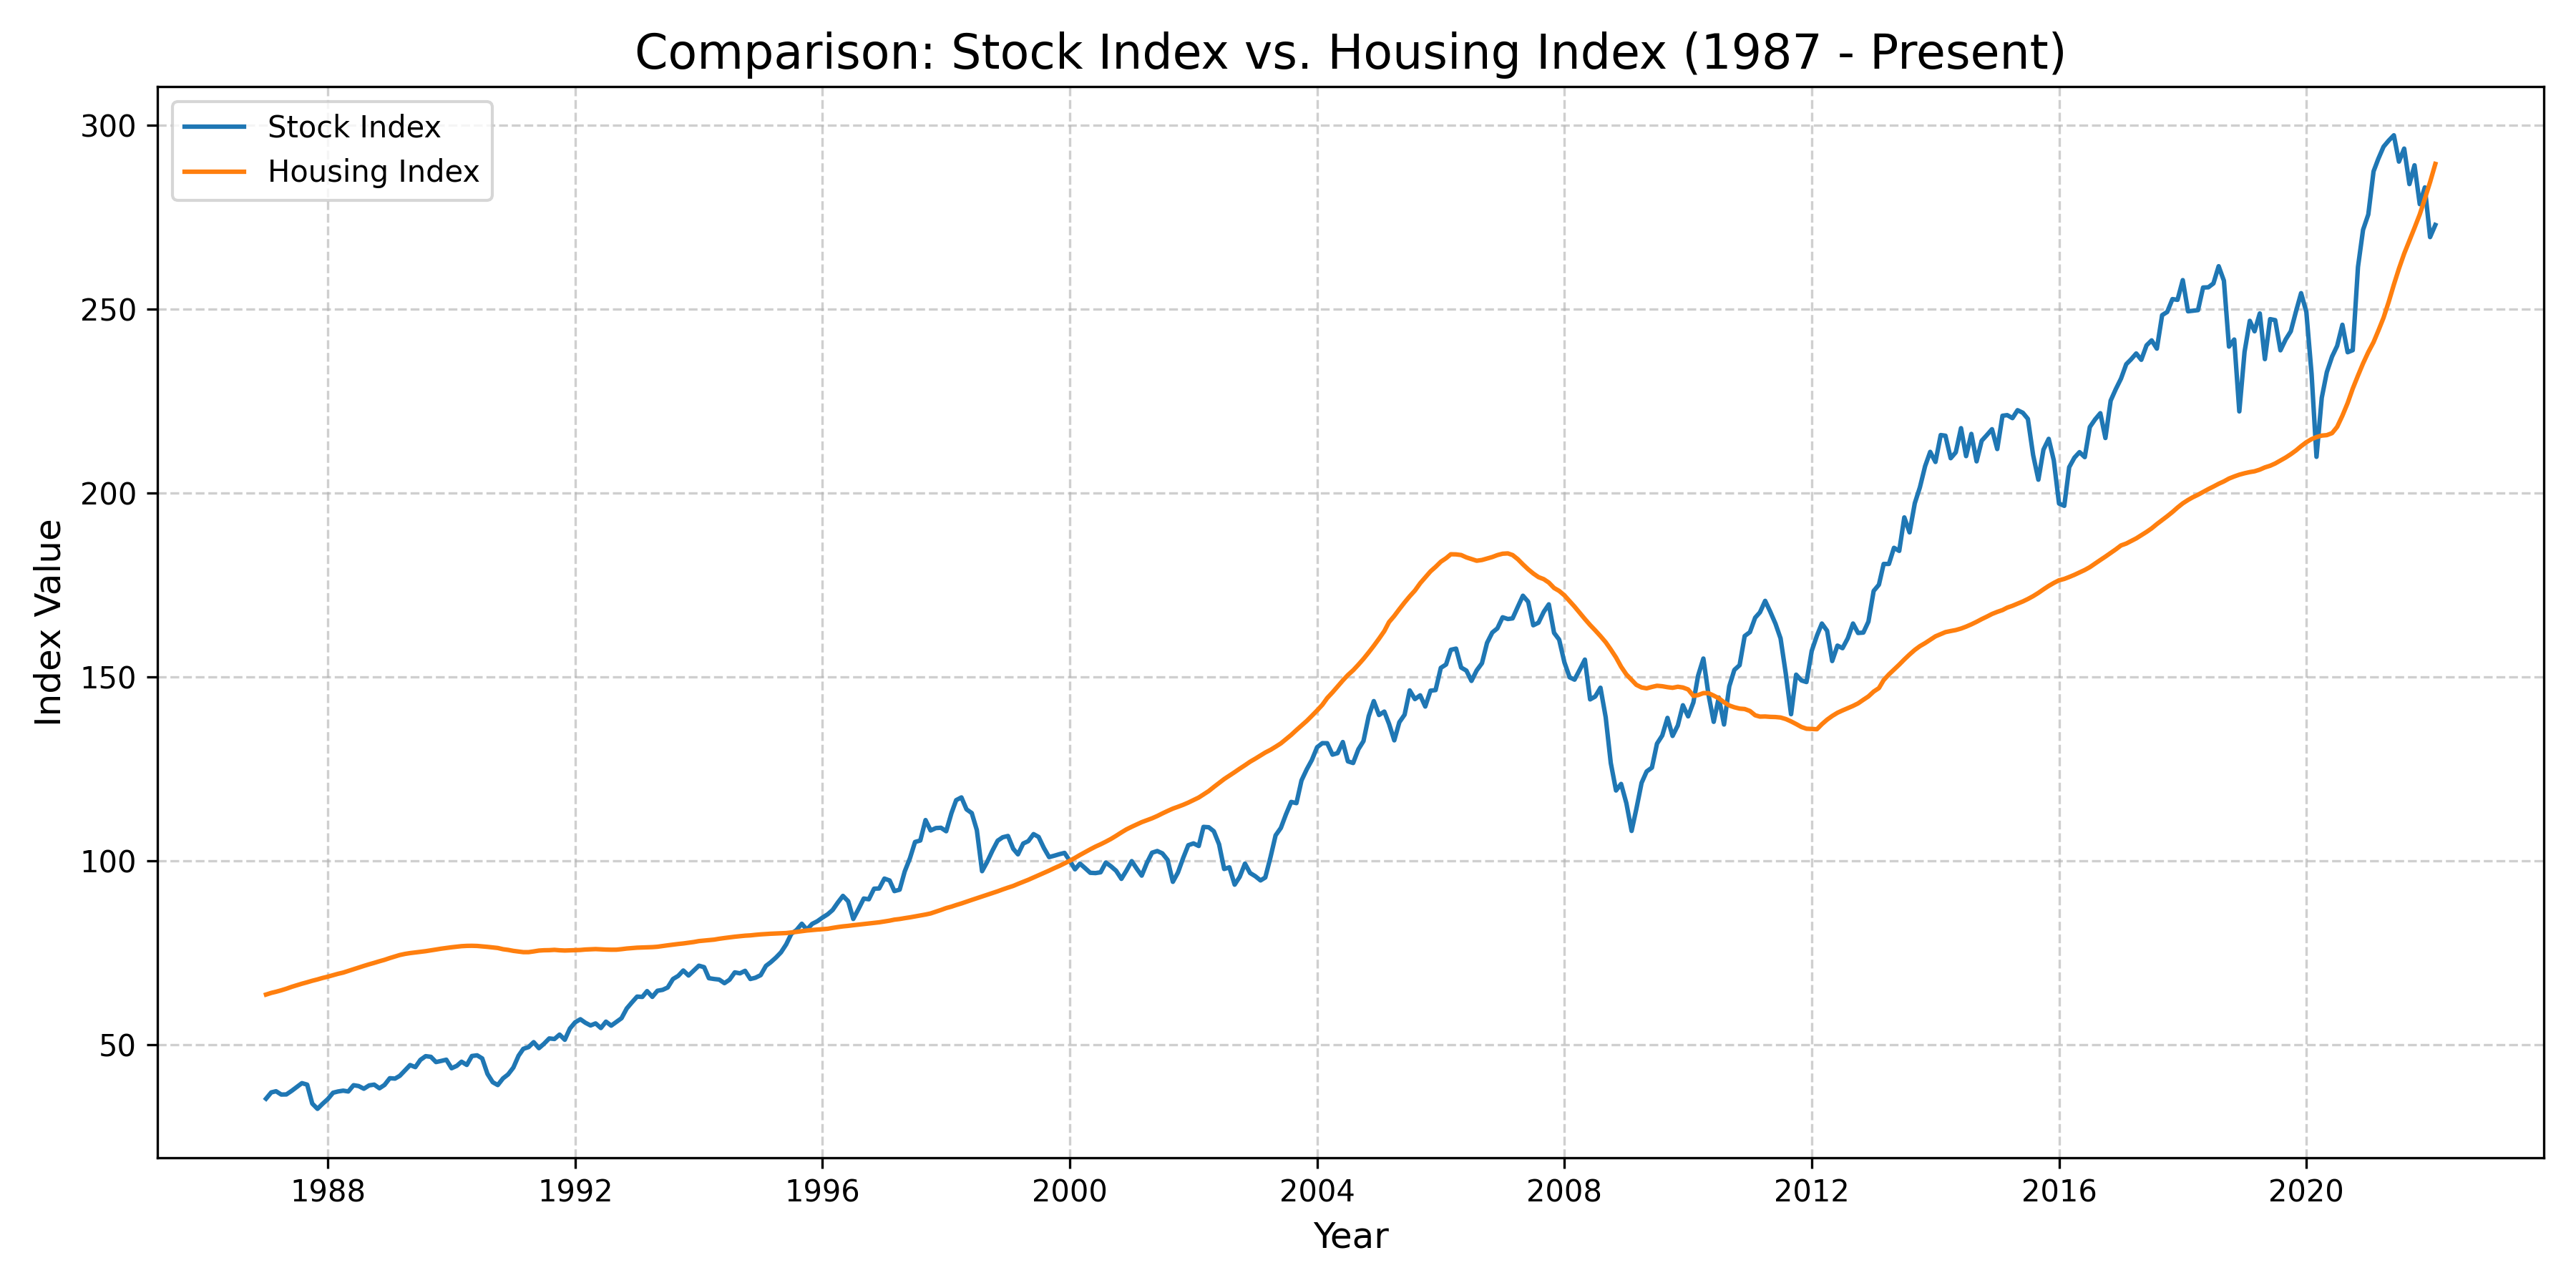
\includegraphics[width=\textwidth]{stock_housing_comparison.png}
  \caption{Comparison of the S\&P 500 stock index against the Case--Shiller U.S.\ National Home Price Index, 1987--present. Both indices exhibit long-run upward trends, but diverge notably during the 2008 financial crisis (housing peaks and collapses while stocks recover faster) and the post-2020 period (housing surges sharply while equity markets remain volatile).}
  \label{fig:index_comparison}
\end{figure}

Table~\ref{tab:top_positive} presents the top 10 most positively correlated assets, filtered to tickers with at least 100 months of overlapping data to exclude statistically unreliable short-history results.

\begin{table}[H]
\centering
\caption{Top 10 most positively correlated assets with the U.S. housing index ($\geq$100 overlapping months).}
\label{tab:top_positive}
\renewcommand{\arraystretch}{1.15}
\small
\begin{tabularx}{\textwidth}{l c r}
\toprule
\textbf{Ticker} & \textbf{Months Compared} & \textbf{Pearson $r$} \\
\midrule
WSBF     & 196 & 0.3553 \\
FTGC     & 100 & 0.3319 \\
HMNF     & 332 & 0.3155 \\
HBP      & 266 & 0.2874 \\
MVBF     & 114 & 0.2838 \\
CELH     & 181 & 0.2660 \\
GBPJPY-X & 218 & 0.2642 \\
CME      & 230 & 0.2640 \\
AAXJ     & 162 & 0.0990 \\
ABCB     & 333 & 0.0985 \\
\bottomrule
\end{tabularx}
\end{table}

The correlation coefficients are uniformly low across all 2,899 assets. The strongest observed value among statistically reliable tickers ($\geq$100 months) is $r \approx 0.36$, and the vast majority fall below $|r| < 0.2$. This is a substantive finding: despite both markets being driven by macroeconomic conditions such as interest rates and GDP growth, they respond to different signals at monthly granularity. As Figure~\ref{fig:index_comparison} illustrates, the 2008 financial crisis caused a sharp divergence --- housing peaked in 2006 and collapsed through 2012, while equity markets recovered far more quickly --- and the post-2020 period saw housing accelerate dramatically while stocks remained volatile. These divergences suppress month-over-month correlation at precisely the most economically interesting periods. Longer-lag analyses or sector-specific groupings (e.g.\ REITs, homebuilders) would likely reveal stronger associations. FX pairs such as \texttt{GBPJPY-X} also appear in the output as they were stored alongside equities in the input directory, and should be excluded in any domain-specific downstream analysis.

% ==========================================================================
\section{Conclusion}
% ==========================================================================

This project demonstrated a complete end-to-end Big Data pipeline for correlating stock market returns with U.S. housing price movements across 3,762 assets and 56.8 million records. A traditional single-node SQL pipeline established a baseline of 5\,m\,39\,s and $\sim$18\,GB peak memory, with 89\% of runtime consumed by sequential file merging and full-table aggregation. A Hadoop MapReduce implementation eliminated the merge step entirely, parallelised aggregation across 3,762 concurrent map tasks, and reduced peak per-container memory to $\sim$2\,GB, achieving a \textbf{3.9$\times$ end-to-end speedup} while producing results consistent with the SQL output.

The gap between the observed speedup and the theoretical maximum from two worker nodes is explained by MapReduce framework overhead (JVM startup, shuffle network I/O) and mild data skew from long-history tickers --- effects that would diminish at larger cluster sizes and data volumes.

The analytical findings indicate that month-over-month stock returns are weakly correlated with housing index changes for the overwhelming majority of assets ($|r| < 0.2$ for most tickers, maximum reliable $r \approx 0.36$). As Figure~\ref{fig:index_comparison} shows, the two markets share long-run trends but diverge sharply at major economic events, suppressing short-term correlation --- consistent with established cross-asset correlation literature at short timescales, and motivating further analysis at longer lags or within specific market sectors.

\end{document}
